\section{What Escaping Costs (RQ4)}
\label{sec:escape}

Suppose the fan with strong preference, three months in and at $V=+\nVStrong$, decides they have seen enough gender group labels but want to keep the topic. What can they do, and at what price?

\paragraph{Set-up.} In the simulation of \cref{sec:sim}, we let the formed user apply one of eleven strategies for 3{,}000 videos (\nActDays{} days) and then stop, returning to their old viewing habits for 4{,}000 more. The strategies cover the main kinds of action open to a user of a short-video app (\cref{tab:escape}): change how they watch (\str{1}, \str{4}, \str{5}), press a button (\str{2}, \str{3}), edit their history (\str{6}, \str{7}), change a platform setting (\str{8}, \str{9}), or put a filter in front of the feed (\str{10}, \str{11}). ``Not interested'' appears twice: as OneRec implements it, with the positive weight measured in \cref{sec:probe} (\str{2}), and as a counterfactual button that the recommender reads as rejection (\str{3}). The filters use the keyword recall of \cref{fig:detection} and the validated classifier. We record the change in skew, the share of the topic kept, the number of explicit actions, and how fast the skew returns.

\begin{table}[t]
\caption{Eleven escape strategies applied by a topic fan with a formed skew of $+\nVStrong$ (means of 400 simulated users). $\Delta V$ is the change in personal skew after 3 and 17 days of acting; ``total'' is the skew relative to supply at day 17, to be compared with the platform layer $+\nPlatformLayer$; ``topic kept'' is the topic share at day 17 relative to before. Effort counts explicit actions per 1{,}000 videos. The last two columns describe the period after the user stops: the remaining change 1{,}000 videos later, and the number of videos until half of the reduction is undone.}
\label{tab:escape}
\centering\small
\setlength{\tabcolsep}{4.2pt}
\begin{tabular}{@{}llrrrrcrr@{}}
\toprule
 & & \multicolumn{2}{c}{$\Delta V$ while acting} & & & & \multicolumn{2}{c}{After stopping}\\
\cmidrule(lr){3-4}\cmidrule(l){8-9}
 & Strategy & 3 days & 17 days & Total & \makecell[r]{Topic\\kept} & Effort & \makecell[r]{$\Delta V$ at\\$+$1{,}000} & \makecell[r]{Half\\undone}\\
\midrule
\tabinput{generated/tab_escape_body}
\bottomrule
\end{tabular}
\end{table}

\begin{figure}[t]
  \centering
  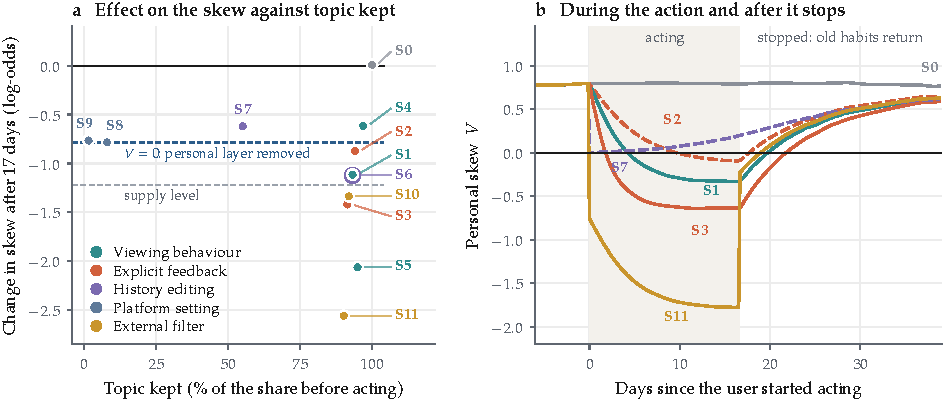
\includegraphics[width=\textwidth]{figures/fig_escape.pdf}
  \caption{Escape. \textbf{(a)} Change in skew after 17 days against the share of the topic kept, for the strategies of \cref{tab:escape}. The upper dashed line is where the personal layer is gone; the lower one is where the platform layer is gone as well. \textbf{(b)} Personal skew before, during and after the action for six strategies. Once the user stops, the curves return towards the old level at a similar pace.}
  \label{fig:escape}
\end{figure}

\paragraph{The controls that platforms offer remove the skew by removing the topic.} Switching personalisation off (\str{8}) sets $V$ to zero at once, and ``show less of this topic'' (\str{9}) gets there in two weeks. Both do it by taking the topic away: 8\% and 2\% of the topic share remains (\cref{fig:escape}a, left). \Cref{prop:topic} explains the second case: a topic-level control cannot change the mix within the topic, and the skew falls only because, with few issue videos left, the narrative drops out of the history. Clearing the whole history (\str{7}) costs half the topic, and its effect starts to wear off while the user is still counted as acting, from $-0.77$ after three days to $-0.62$ after seventeen, because habits that have not changed rebuild the skew. None of the three goes below the platform layer ($+0.44$ to $+0.60$ in total), in line with \cref{prop:reach}.

\paragraph{Narrative-level actions keep the topic, but the user has to do the work.} Scrolling past group-label videos (\str{1}) lowers the skew by 1.11 and keeps 93\% of the topic. Deleting those videos from the history first (\str{6}) reaches the same level within three days where scrolling alone takes two weeks. Adding a search for rebuttal videos to scrolling past (\str{5}) goes furthest of the behavioural strategies ($-2.06$), at the price of 30 searches per 1{,}000 videos. Simply finishing more of the ordinary issue videos (\str{4}) helps least ($-0.62$): an ordinary video is weak evidence about the narrative, so it takes many of them to offset one group-label video. All of these except \str{4} push $V$ below zero. The user then ends up below the platform layer only by making the recommender believe they dislike the narrative, a state that their underlying preference does not support.

\paragraph{The button does worse than doing nothing with the video.} \str{1} and \str{2} differ in one respect only: in both the user stops finishing group-label videos, and in \str{2} they also press ``not interested''. Pressing the button as implemented is less effective than scrolling past without a word: $-0.34$ against $-0.58$ after three days, $-0.87$ against $-1.11$ after seventeen, for 21 presses per 1{,}000 videos. Each press tells the recommender, with about two-fifths of the weight of a finished video, that this kind of video matters to the user. If the button were read as rejection (\str{3}), the same presses would make it the best explicit tool ($-1.42$, 91\% of the topic kept). The loss of topic is small because the narrative contrast is large relative to the topic contrast; the exchange rate $t/c$ of \cref{prop:feedback} is favourable for this narrative and would be worse for one the recommender separates less clearly.

\paragraph{Filters reach furthest and need no cooperation from the recommender.} The classifier filter (\str{11}) lowers the skew by 2.01 within three days and 2.56 after seventeen, taking the user well below supply level while keeping 90\% of the topic; the keyword list (\str{10}) achieves $-1.34$. \Cref{prop:filter} gives the direct effects as $\log\frac{0.21}{0.99}=-1.55$ and $\log\frac{0.55}{0.99}=-0.59$. The remainder is indirect: videos that never reach the screen are never finished, so the recommender's own estimate of the user's taste drifts down as well.

\paragraph{Nothing lasts.} When the user stops, the skew returns under every strategy (\cref{fig:escape}b). For every strategy that kept 90\% or more of the topic, half of the reduction is gone after 1{,}200 to 1{,}500 videos, about a week; after clearing the history it takes about 2{,}200 videos, or twelve days. After 4{,}000 videos all of these are back within 0.3 of the starting level. The two platform settings stay low for longer only because the topic itself must first grow back. The recommender has a memory of about 200 finished videos. No single action leaves a lasting mark on it, and the preference that produced the skew is still there. Escape is therefore not an act but a habit, and the realistic choice is between a filter that works unattended and a change in what one finishes.
